\documentclass[12pt, titlepage]{article}

\usepackage{longtable}
\usepackage{booktabs}
\usepackage{tabularx}
\usepackage[shortlabels]{enumitem}
\usepackage{hyperref}
\hypersetup{
    colorlinks,
    citecolor=blue,
    filecolor=black,
    linkcolor=red,
    urlcolor=blue
}
\usepackage[round]{natbib}
\usepackage{amsmath}
\usepackage{array}
\usepackage{graphicx}


\input{../Comments}
%% Common Parts

\newcommand{\progname}{Room8} % PUT YOUR PROGRAM NAME HERE
\newcommand{\authname}{Team 19
\\ Mohammed Abed
\\ Maged Armanios
\\ Jinal Kasturiarachchi
\\ Jane Klavir
\\ Harshil Patel} % AUTHOR NAMES

\usepackage{hyperref}
    \hypersetup{colorlinks=true, linkcolor=blue, citecolor=blue, filecolor=blue,
                urlcolor=blue, unicode=false}
    \urlstyle{same}
                                


\begin{document}

\title{System Verification and Validation Plan for \progname{}} 
\author{\authname}
\date{2024-11-04}
	
\maketitle

\pagenumbering{roman}

\section*{Revision History}

\begin{tabularx}{\textwidth}{p{3cm}p{2cm}X}
\toprule {\bf Date} & {\bf Version} & {\bf Notes}\\
\midrule
2024-11-04 & 0.0 & Document Created\\
\bottomrule
\end{tabularx}

~\\


\newpage

\tableofcontents

\listoftables

\listoffigures

\newpage

\section{Symbols, Abbreviations, and Acronyms}

\renewcommand{\arraystretch}{1.2}
\begin{tabular}{l l} 
  \toprule		
  \textbf{Acronym} & \textbf{description}\\
  \midrule 
  SRS & Software Requirements Specification\\
  VnV & Verification and Validation\\
  CI/CD & Continuous Integration and Continuous deployment\\   
  API & Application Programming Interface\\
  \bottomrule
\end{tabular}\\

\newpage

\pagenumbering{arabic}

This document provides the VnV plans for all relevant aspects of this project. These include the VnV plans for the SRS, system architecture, implementation, and requirements. In addition, this document outlines the expected software and tools to be used in the VnV and the expected roles/responsibilities of the project team. \\\\This document begins with a 
\hyperref[sec:generalInfo]{General Information Section} that acts as a primer to the project and contains all the background information needed to understand the document.\\\\Following the primer, \hyperref[section:JustPlan]{Section 3} outlines the VnV plans for project and is followed by \hyperref[section:systemTests]{System Tests} for all the requirements outlined in the SRS. In future revisions, a 5th section outlining detailed unit tests will be added to this document, but at the time of writing the detailed design had not been completed.

\section{General Information}
\label{sec:generalInfo}
\subsection{Summary}

Shared living environments often create tension between roommates. It can be inconvenient and sometimes awkward to explicitly reach out to a roommate about the messes they leave behind in a shared space, concerns over bill payments, household upkeep, and more. Our project, Room8,
aims to prevent these cumbersome interactions by providing an application and the
necessary hardware components to help monitor the cleanliness of shared spaces,
schedule tasks, track shared billing cycles, and alert roommates of any issues within the shared house.

\subsection{Objectives}


The objective for this document, and the VnV plan that it outlines, is to support the idea that all software built for the project is correct, complete, and provides a satisfying user experience. The reason why these qualities are emphasized are due to the fact that the outputs of our system have real-life implications (i.e. cleanliness detector determining the incorrect roommate made a mess, bill splitter incorrectly calculating amounts due, etc.), making correctness and completion essential. Additionally, since the application is very user-centric, the user experience is central to the project's success and must be treated as such. Since this will be the main focus of our testing efforts, there are certain elements of our project which will not be tested extensively by our own team. For example, any external libraries that will be used as a part of Room8 will be assumed to have rigorous verification and validation already completed by the implementation team who created it. Additionally, extreme scalability/load testing will not be completed as part of the initial VnV. This is due to the hypothetical nature of the project in its current state, which doesn't require the system to be able to withstand many concurrent users at a time. 

\subsection{Challenge Level and Extras}


The challenge level of our project is general. The extras that will be completed as part of this project include additional features related to student housing and user documentation. Since the main functionality of Room8 is the cleanliness detector and image processing is not a novel concept (mess detecting software already exists), the challenge level is not advanced. However, the program still presents a variety of difficulties on the implementation side, preventing it from being classified as basic. The extras include the user-facing software, which provides all of the other student housing features (i.e. bill splitter, scheduler, etc.), and a thorough guide for the application and installation of the hardware will be delivered upon the project's completion.  

\subsection{Relevant Documentation}
The SRS will be referenced throughout the VnV process, as it contains all of the system requirements, which will be verified and validated through testing. Every requirement in the SRS will be referenced by one or more test(s) in this document to ensure that the system is functioning as expected and that everything required from the system is being completed.

\section{Plan}
\label{section:JustPlan}
The following section outlines the execution plan for verifying project documentation and validating the software. The sections begin outlining the verification and validation team. Following section 3.1, sections 3.2 and 3.4 outline the plans for verifying documentation, while sections 3.5-3.7 discuss verification and validation for the system.

\subsection{Verification and Validation Team}
\begin{longtable}{|>{\raggedright\arraybackslash}p{0.21\linewidth} | >{\raggedright\arraybackslash}p{0.21\linewidth} | >{\raggedright\arraybackslash}p{0.60\linewidth}| >{\raggedright\arraybackslash}p{0.21\linewidth}| }
    \caption{\bf Verification and Validation Team} \label{tab:my_label} \\
    
    \hline
    \textbf{Teammate} & \textbf{Position} & \textbf{Project Role}\\
    \hline
    \endfirsthead
    
    \hline
    \textbf{Teammate} & \textbf{Position} & \textbf{Project Role}\\
    \hline
    \endhead
    
    \hline
    \endfoot
    
    \hline
    \endlastfoot


    \hline
    Mohammed Abed & Developer & Mohammed's role will be focused on automating test cases using online tools such as GitHub actions and any other tools the team chooses to use. Since Mohammed's strengths and past experiences are in web development, he will also provide support in developing tests for the user-facing application. \\
   	\hline
    Maged Armanios & Developer & Maged's role will focus on developing unit and usability tests for the user-facing application and its backend. These tests will be then automated by Mohammed using tools like GitHub Actions. \\
    \hline
    Jinal Kasturiarachchi & Developer & Jinal will verify the usability requirements for the system. In addition, due to the expected workload of each role being unknown at the time of writing, Jinal will support any other developer who has received a larger-than-average workload. \\
    \hline
    Jane Klavir & Developer & Jane's role will have her verify the cleanliness management system meets the requirements outlined. This includes that it'll be able to detect created messes, cleaned messes, and states of no change. \\
    \hline
    Harshil Patel & Developer & Harshil will focus on testing the safety and security of the system. This includes ensuring all data is stored securely, access tokens are confidential, and authorization is secure on the user's end.  \\
	\hline
	Dr. R Tharmarasa & Supervisor & Dr. Tharmarasa's role will be to provide the team with support in making decisions related to the cleanliness management algorithm. Additionally, Dr. Tharmarasa will provide his input on the feasibility of requirements related to the cleanliness management system using his research experience in classification and related topics.
\end{longtable}

\textbf{Note about project roles}: While each team member has specific roles, all members of the team are expected to be able to support each other when required. The roles defined in the table above are simply the optimal roles for each member based on their expertise and do not restrict the work they are able to undergo to only what's outlined in the table above.

\subsection{SRS Verification Plan}
\label{section:SRSVerificationPlan}
To verify our SRS, the development team will meet with the project supervisor, dr. Tharmarasa. In this meeting, the group will present a summarized version of the SRS which outlines the components, functionality, constraints, and assumptions. This presentation will be accompanied by some form of presentation of the use-case scenarios outlined in the SRS. This can be done with either a low-fidelity mock-up or a live demo of the system if sufficient development has been completed. After the presentation, we will ask the supervisor whether they found any use cases unimportant and requirements unverifiable. After meeting with our supervisor, the team will redraft the requirements and use cases according to his feedback. \\\\
In the event we are unable to meet with our supervisor for review, an alternative approach would be to seek peer review and feedback from our primary project reviewers. The meeting would have a similar structure to that which, would be done with Dr. Tharmarasa. \\

Additionally, the development team will review the SRS document to verify each requirement:
\begin{itemize}
\item Is free of implementation details
\item Does not include acceptance criteria
\item Does not conflict with any other requirement
\end{itemize}


\subsection{Design Verification Plan}
The system architecture will be verified by the development team in a formal meeting. The meeting will have each member read through the system architecture and verify it according to the following checklist:
\begin{itemize}
\item For each requirement and/or use case defined in the SRS, does the architecture enable the system to do so?
\item Is there no overlap between the modules (separation of concerns)?
\item Is the system easy to scale (consider both horizontal and vertical scaling)? If you were to scale the system, how would you do so?
\item Does the architecture include security measures to satisfy the non-functional requirements in the SRS?
\item Does the architecture support unit testing?
\item Does the architecture support the addition of new modules (extension)? 
\end{itemize}

\subsection{Verification and Validation Plan Verification Plan}
The Verification and Validation Plan will be read by each member of the team to confirm the following:
\begin{itemize}
\item Each teammember referenced has clear, defined roles with a clause for role switching and overlapping roles
\item Each test satisfies the following:
\begin{itemize}
\item The test corresponds to a requirement in the SRS
\item Functional requirements have test cases specific enough that a test can be built with the data. Including clearly defined inputs and outputs
\item Functional test cases are deterministic
\item Nonfunctional test cases are specific and provide enough information that someone can run the test once the product is built. 
\end{itemize}

\end{itemize}




\subsection{Implementation Verification Plan}
The system implementation will be verified using a plethora of tools and techniques. First, the implementation of the system will be verified using the \hyperref[section:systemTests]{system tests} and \hyperref[section:unitTests]{unit tests} outlined in sections \hyperref[section:systemTests]{4} and 5 (5 is omitted until the detailed design is complete). Additionally, the development team will create integration tests to see if the interactions between different modules are expected. Any tests that can be used during CI/CD use will be done with them to ensure changes to the source code do not create a loss of functionality. Finally, the team will perform an acceptance test, running the application and acting out the key use-case scenarios outlined in the SRS.\\
\\
During development, the team will use static analysis tools to help minimize common development mistakes such as referencing non-existent variables, incorrect type operations, etc.\\
\\ Additional tests that can be executed if required are:
\begin{itemize}
\item Code walkthroughs with the development team
\item Review sessions with our team's primary reviewers
\end{itemize}

\subsection{Automated Testing and Verification Tools}
\label{subsec:tools}
At the time of writing, the programming languages have not been finalized. Nonetheless, this section outlines the expected tools that will be utilized for the expected programming languages and frameworks. Currently, the expected programming languages and frameworks are expected to be JavaScript/TypeScript for the frontend application, utilizing the React framework, and Python for the cleanliness management system.
  
  \textbf{TypeScript}:
   \begin{itemize}
   \item Jest: The preferred framework for testing React-based applications
   \item Puppeteer: Provides high-level APIs to control Chrome and allows for automating UI testing, form submissions, and keyboard inputs easily
   \item ESLint: A code linter that helps catch common programming mistakes and can be enhanced to enforce code styling. Automates the detection of potential vulnerabilities and life-cycle methods for React-based projects.
   \end{itemize}
   \textbf{Python}:
   \begin{itemize}
   \item Pylance: A language server providing tools features like IntelliSense, logical linting, code actions, code navigation, and semantic colorization. These features can assist developers in catching errors while developing.
   \item Flake8: A command-line utility for enforcing style consistency across Python projects. Includes lint checks.
   \item Pytest and PyUnit: Testing frameworks.
   \end{itemize}
  \textbf{CI/CD Tools}:
  \begin{itemize}
  \item GitHub Actions: Allows for the automation of builds and tests
  \end{itemize}
    \textbf{API Testing Tools}:
  \begin{itemize}
  \item Postman: Can run API functional and performance tests to determine average and median API response times. Postman can also be used to ensure the correctness of an API's response 
  \end{itemize}

\subsection{Software Validation Plan}
In the \hyperref[section:SRSVerificationPlan]{SRS verification plan}, a meeting with the project supervisor, dr. Tharmarasa was mentioned, which had him review the use cases and requirements of the project. This session will also act as part of the software validation plan since Dr. Tharmarasa is independent of the development and project team. Additionally, feedback from primary reviewers and primary stakeholders (people living in shared living spaces) will be taken into consideration and possibly used to revise some requirements.    
\section{System Tests}
\label{section:systemTests}
This section outlines the tests that will be used to verify and validate that Room8 is meeting its requirements. \hyperref[subsec:testsForFunc]{4.1} and \hyperref[subsec:testsForNonFunc]{4.2} designate tests for functional and nonfunctional requirements respectively, and tests are furthermore split into Room8's various modules for ease of readability and traceability. The output section of each test case describes the pass condition, thus this is the criteria the app developers will use to confirm that the app aligns with requirements. 

\subsection{Tests for Functional Requirements}
\label{subsec:testsForFunc}
Functional requirements pertain to the core functionality of the app. Room8 has the core functionality of registering users into a home, deploying a ChatBot for notifications, establishing a cleanliness managegement system, providing an event scheduler, and implementing a bill-splitter. The following tests will provide evidence of these integral components being successfully fulfilled.

\subsubsection{User Authentication and House Management}
When a group of students chooses to adopt Room8 to help with their house, the first step is to register all the members and connect them into a common home group through the app. The tests in this section realize this fundamental first step, and are in conjunction with requirements FR211-FR218.

\renewcommand{\arraystretch}{1.5}
\begin{center}
  \testcase{
    \textbf{FST-UAHM-1} & \textbf{Profile Creation}\\\hline

    \textbf{Description} & Tests if the system is able to handle creating user profiles in the system from frontend inputs \\ 

    \textbf{References} & FR211 \\ 

    \textbf{Type} & System Test (dynamic, automated) \\ 

    \textbf{Initial State} & Frontend inputs are empty. User profile does not exist in the system \\ 

    \textbf{Input} & Unique testing email, any name, any password \\ 

    \textbf{Output} & User profile entry is created in the system using the inputted email, name, and password. Frontend redirects user to the dashboard\\ 

    \textbf{Procedure} & Testing agent navigates to the account creation page of the application. Agent enters a unique testing email address, any name, and any password. Agent submits account creation  \\ 
  }

  \testcase{
    \textbf{FST-UAHM-2} & \textbf{System Login}\\\hline

    \textbf{Description} & Tests if the system is able to recognize a user profile and to authenticate them to the system \\ 

    \textbf{References} & FR212 \\ 

    \textbf{Type} & System Test (dynamic, automated) \\ 

    \textbf{Initial State} & Testing profile exists in the system. System does not have the profile currently authenticated \\ 

    \textbf{Input} & Valid email and password matching the profile in the system \\ 

    \textbf{Output} & User profile is authenticated with a new session entry. Frontend redirects user to the dashboard \\ 

    \textbf{Procedure} & Testing agent navigates to the account login page of the application. Agent enters a valid testing account email address and password. Agent submits account login  \\ 
  }

  \testcase{
    \textbf{FST-UAHM-3} & \textbf{System Logout}\\\hline

    \textbf{Description} & Tests if the system logs the user out, invalidating their session and returning them to the homepage \\ 

    \textbf{References} & FR213 \\ 

    \textbf{Type} & Functional Test (dynamic, automated) \\ 

    \textbf{Initial State} & Testing profile is logged in with an active session \\ 

    \textbf{Input} & User clicks on the logout button \\ 

    \textbf{Output} & The system invalidates the session and redirects the user to the homepage \\ 

    \textbf{Procedure} & Testing agent clicks the logout button and confirms that the user is logged out and redirected to the homepage \\ 
  }

  \testcase{
    \textbf{FST-UAHM-4} & \textbf{Create Home Instance}\\\hline

    \textbf{Description} & Tests if the system allows users to create a new home group with specified details \\ 

    \textbf{References} & FR214, FR216 \\ 

    \textbf{Type} & System Test (dynamic, automated) \\ 

    \textbf{Initial State} & User is logged in, and no home group exists for their account \\ 

    \textbf{Input} & Home name, address, and number of roommates \\ 

    \textbf{Output} & A new home group instance is created with the specified details, and the user is added as a member \\ 

    \textbf{Procedure} & Testing agent navigates to the home creation page, enters the home name, address, and number of roommates, and submits the form. Confirm that the home instance is created and the user is added as a member \\ 
  }

  \testcase{
    \textbf{FST-UAHM-5} & \textbf{Invite and Remove Users From Home Instance}\\\hline

    \textbf{Description} & Tests if the system allows users to invite others to join a home group and remove them as needed \\ 

    \textbf{References} & FR215, FR217, FR218 \\ 

    \textbf{Type} & Integration Test (dynamic, automated) \\ 

    \textbf{Initial State} & A home group exists with only the logged-in user as a member \\ 

    \textbf{Input} & Valid email address of another user to invite; selection of a user to remove \\ 

    \textbf{Output} & The invited user receives an invitation, joins the home group upon acceptance, and can be removed by the home admin \\ 

    \textbf{Procedure} & Testing agent invites another user via their email. Once accepted, confirm the user is added to the home group. Then, the agent removes the user and confirms their removal from the group. \\ 
  }
  
  \testcase{
    \textbf{FST-UAHM-6} & \textbf{Leave Home Instance}\\\hline

    \textbf{Description} & Tests if the system allows users to leave a home group as needed \\ 

    \textbf{References} & FR216, FR218 \\ 

    \textbf{Type} & Functional Test (dynamic, automated) \\ 

    \textbf{Initial State} & A home group exists with user as a member \\ 

    \textbf{Input} & ID of a home group to leave\\ 

    \textbf{Output} & User receives feedback on their action to leave the home group \\ 

    \textbf{Procedure} & Testing agent views home group then selects the option to leave the home group. The testing agent then verifies that the user has left the home group. \\ 
  }

\end{center}

\subsubsection{ChatBot Configuration}
The ChatBot is configured to send necessary reminders and notifications to the group. To ensure the ChatBot is accomplishing its role, the following tests for FR221-FR224 will be used.

\begin{center}
  \testcase{
    \textbf{FST-CC-1} & \textbf{Update Chatbot Settings}\\\hline

    \textbf{Description} & Tests if the chatbot settings can be updated successfully by an authorized user \\ 

    \textbf{References} & FR221 \\ 

    \textbf{Type} & Functional Test (dynamic, automated) \\ 

    \textbf{Initial State} & Chatbot is configured with default settings \\ 

    \textbf{Input} & Randomized array of include and exclude inputs \\ 

    \textbf{Output} & ChatBot settings entry in database reflect the array of inputs \\ 

    \textbf{Procedure} & Testing agent navigates to the chatbot settings page, iterates through each setting checkbox corresponding to randomized boolean input array. Agent saves changes. Database is verified to contain the updated array of inputs \\ 
  }

  \testcase{
    \textbf{FST-CC-2} & \textbf{GroupChat Created with ChatBot}\\\hline

    \textbf{Description} & Tests if all users attached to a home instance are added to a groupchat alongside the ChatBot \\ 

    \textbf{References} & FR225 \\ 

    \textbf{Type} & Integration Test (dynamic, manual) \\ 

    \textbf{Initial State} & Agent has user profile and is part of a home instance with more than 2 users linked. Chatbot phone number is not present in the group chat. ChatBot has no corresponding groupchat entry \\

    \textbf{Input} & User clicks "Create GroupChat" button \\ 

    \textbf{Output} & All users are added to the group chat alongside the ChatBot \\ 

    \textbf{Procedure} & Testing agent navigates to the group chat creation page and clicks the "Create GroupChat" button. Agent verifies that all users are added to the group chat alongside the ChatBot \\
  }

  \testcase{
    \textbf{FST-CC-3} & \textbf{ChatBot Sends Messages to Groupchats}\\\hline
    
    \textbf{Description} & Tests if the ChatBot is able to send messages to a group chat as per configuration \\ 

    \textbf{References} & FR222, FR223, FR224\\ 

    \textbf{Type} & System Test (dynamic, automated) \\ 

    \textbf{Initial State} & Chatbot is added to a group chat with configured message triggers \\ 

    \textbf{Input} & New database entry created for a chore, cleanliness score, and a shared expense \\ 

    \textbf{Output} & Chatbot sends the appropriate configured messages to the group chat \\ 

    \textbf{Procedure} & Testing agent creates a new database entry for a chore, cleanliness score, and a shared expense. Agent verifies that the ChatBot sends the appropriate messages to the group chat according to the configured ChatBot settings\\
  }

\end{center}

\subsubsection{Cleanliness Manager}
The cleanliness manager is the unique selling point of the Room8 app. It assesses the cleanliness of spaces by running an algorithm to output an objective cleanliness score. To ensure this functionality is working properly (i.e. FR231-FR235), the following tests are used.

\begin{center}
  \testcase{
    \textbf{FST-CM-1} & \textbf{System Evaluates Cleanliness}\\\hline

    \textbf{Description} & Tests if the system can evaluate and record cleanliness scores based on captured images \\ 

    \textbf{References} & FR231 \\ 

    \textbf{Type} & System Test (dynamic, manual) \\ 

    \textbf{Initial State} & Cleanliness management camera is setup and connected to home instance \\ 

    \textbf{Input} & N/A \\ 

    \textbf{Output} & Cleanliness scores are updated based on user actions \\ 

    \textbf{Procedure} & Home resident enters camera view and creates a mess. Resident verifies that the cleanliness score is updated to reflect the mess. Resident then cleans the mess and verifies that the cleanliness score is updated to reflect the clean state \\ 
  }

  \testcase{
    \textbf{FST-CM-2} & \textbf{Display Cleanliness Scores}\\\hline

    \textbf{Description} & Tests if the system displays cleanliness scores to users in a group \\ 

    \textbf{References} & FR232, FR233, FR234, FR235 display requirements \\ 

    \textbf{Type} & Functional Test (dynamic, automated) \\ 

    \textbf{Initial State} & Cleanliness scores are available for the group \\ 

    \textbf{Input} & N/A \\ 

    \textbf{Output} & Cleanliness scores are displayed accurately to the user \\ 

    \textbf{Procedure} & Testing agent navigates to the cleanliness score display page and verifies that the scores are shown accurately \\ 
  }

\end{center}

\subsubsection{Schedule Configuration}
Room8 provides a convenient calendar to allow users to schedule chores and events and stay organized, as outlined by requirements FR241-FR245. The tests here will be used to ensure this component of the app is functioning correctly.

\begin{center}
  \testcase{
    \textbf{FST-CM-1} & \textbf{System Evaluates Cleanliness}\\\hline

    \textbf{Description} & Tests if the system can evaluate and record cleanliness scores based on captured images \\ 

    \textbf{References} & FR231 \\ 

    \textbf{Type} & System Test (dynamic, manual) \\ 

    \textbf{Initial State} & Cleanliness management camera is setup and connected to home instance \\ 

    \textbf{Input} & N/A \\ 

    \textbf{Output} & Cleanliness scores are updated based on user actions \\ 

    \textbf{Procedure} & Home resident enters camera view and creates a mess. Resident verifies that the cleanliness score is updated to reflect the mess. Resident then cleans the mess and verifies that the cleanliness score is updated to reflect the clean state \\ 
  }

  \testcase{
    \textbf{FST-CM-2} & \textbf{Display Cleanliness Scores}\\\hline

    \textbf{Description} & Tests if the system displays cleanliness scores to users in a group \\ 

    \textbf{References} & FR232, FR233, FR234, FR235 \\ 

    \textbf{Type} & Functional Test (dynamic, automated) \\ 

    \textbf{Initial State} & Cleanliness scores are available for the group \\ 

    \textbf{Input} & N/A \\ 

    \textbf{Output} & Cleanliness scores are displayed accurately to the user \\ 

    \textbf{Procedure} & Testing agent navigates to the cleanliness score display page and verifies that the scores are shown accurately \\ 
  }

\end{center}

\subsubsection{Schedule Configuration}
Room8 provides a convenient calendar to allow users to schedule chores and events and stay organized, as outlined by requirements FR241-FR245. The tests here will be used to ensure this component of the app is functioning correctly.

\begin{center}
  \testcase{
    \textbf{FST-SC-1} & \textbf{Adding Event to Schedule}\\\hline

    \textbf{Description} & Tests that new event appears in calendar after it is inputted. \\ 

    \textbf{References} & FR241, FR242, FR243, FR245 \\ 

    \textbf{Type} & Functional Test (dynamic, automated) \\ 

    \textbf{Initial State} & Calendar displaying chores and events pertaining to the house. \\ 

    \textbf{Input} & Title, date, time, and duration. \\ 

    \textbf{Output} & Calendar displaying new chore/event with input parameters.  \\ 

    \textbf{Procedure} & Testing agent navigates to calendar, generates a series of events with random inputs, and adds them to the schedule. Agent verifies that the events with the same input parameters exist in the schedule.  \\ 
  }

    \testcase{
      \textbf{FST-SC-2} & \textbf{Removing Event from Schedule}\\\hline
  
      \textbf{Description} & Tests that event disappears from calendar after existing event is removed. \\ 
  
      \textbf{References} & FR244 \\ 
  
      \textbf{Type} & Functional Test (dynamic, automated) \\ 
  
      \textbf{Initial State} & Calendar displaying chores and events pertaining to the house. \\ 
  
      \textbf{Input} & Chore/event from calendar represented by name, date, time, and duration. \\ 
  
      \textbf{Output} & Chore/event that was removed is no longer displayed in its previous timeblock in the calendar. \\ 
  
      \textbf{Procedure} & Testing agent navigates to calendar, and removes the series of events it generated in FST-SC-1. Agent verifies that the events it removed do not exist in the schedule.  \\ 
    }

      \testcase{
        \textbf{FST-SC-3} & \textbf{Editing Event in Schedule}\\\hline
    
        \textbf{Description} & Tests that changes can be made to an already-existing event. \\ 
    
        \textbf{References} & FR244 \\ 
    
        \textbf{Type} & Functional Test (dynamic, automated) \\ 
    
        \textbf{Initial State} & Calendar displaying chores and events pertaining to the house. \\ 
    
        \textbf{Input} & Chore/event from calendar represented by name, date, time, and duration. \\ 

        \textbf{Output} & Chore/event displayed in calendar after edits contains updated information (i.e. name, date, time, and/or duration).  \\
    
        \textbf{Procedure} & Testing agent navigates to calendar, and adds an event with random input. Then, testing agent edits that event by changing name, date, time, and duration one-by-one, verifying each time that the parameter edited has changed. Then, testing agent edits 2 random parameters simultaneously, then 3 random parameters simultaneously, and finally all the parameters simultaneously, verifying after each step. \\ 
      }


  \testcase{
    \textbf{FST-SC-4} & \textbf{Display Event Schedule}\\\hline

    \textbf{Description} & Tests that all events displayed in calendar view. \\ 

    \textbf{References} & FR245 \\ 

    \textbf{Type} & Functional Test (dynamic, automated) \\ 

    \textbf{Initial State} & User is logged in and registered in home group \\ 

    \textbf{Input} & User requests to view calendar \\ 

    \textbf{Output} & Calendar displaying chores and events pertaining to the home group \\ 

    \textbf{Procedure} & Testing agent navigates to calendar and confirms that chores and events are displayed accurately. \\ 
  }

\end{center}

\subsubsection{Bill Splitter Configuration}
Various expenses will inevitably accumulate for a group of roommates. The bill splitter keeps track of expenses and amounts owed by each member. The Room8 app must be able to deal with expenses accurately (as covered by FR251-FR255) and these tests will serve as confirmation.

\begin{center}
  \testcase{
    \textbf{FST-BSC-1} & \textbf{Add and Split Expense}\\\hline

    \textbf{Description} & Tests if the system allows users to add a new expense and splits it among group members \\ 

    \textbf{References} & FR251 \\ 

    \textbf{Type} & System Test (dynamic, automated) \\ 

    \textbf{Initial State} & No expenses recorded for the current month \\ 

    \textbf{Input} & New expense with an amount and shared expense roommates \\ 

    \textbf{Output} & Expense is split equally among group members and recorded \\ 

    \textbf{Procedure} & Testing agent navigates to the add expense page, enters details, and verifies that the expense is split among group members \\ 
  }

  \testcase{
    \textbf{FST-BSC-2} & \textbf{Display User Expenses}\\\hline

    \textbf{Description} & Tests if the system displays all expenses associated with a user \\ 

    \textbf{References} & FR252, FR253. FR255 \\ 

    \textbf{Type} & Functional Test (dynamic, automated) \\ 

    \textbf{Initial State} & Recorded expenses are available in the system \\ 

    \textbf{Input} & User navigates to their expenses page \\ 

    \textbf{Output} & System displays all expenses associated with the user \\ 

    \textbf{Procedure} & Testing agent navigates to the user expenses page and verifies that all expenses are displayed correctly \\ 
  }
  
   \testcase{
    \textbf{FST-BSC-3} & \textbf{Mark Expense as Paid}\\\hline

    \textbf{Description} & Tests if the system allows users to mark an expense as paid \\ 

    \textbf{References} & FR253, FR254 \\ 

    \textbf{Type} & Functional Test (dynamic, automated) \\ 

    \textbf{Initial State} & An unpaid expense is available in the system \\ 

    \textbf{Input} & User navigated to an expenses page and marks an expense as paid \\ 

    \textbf{Output} & System updates the UI state and displays all expenses associated with the user \\ 

    \textbf{Procedure} & Testing agent navigates to the user expenses page and marks an expense as paid. The system then refreshes the UI and the testing agent will verify that the marked expense is displayed as paid\\ 
  }

\end{center}

\subsection{Tests for Nonfunctional Requirements}
\label{subsec:testsForNonFunc}
Nonfunctional requirements are the quality attributes of the system. Covering nonfunctional requirements ensures that Room8 is operating well, and this subsection contains such tests for the nonfunctional requirements outlined in the SRS.

\subsubsection{Area of Testing: User Authentication and House Management}
This section covers encryption standards for authentication and house management data of the application, as presented in SRS, Section S.2.1.

\renewcommand{\arraystretch}{1.5}
\begin{center}
  \testcase{
		\textbf{NFST-UAHM-1} & \textbf{Encryption of Authentication Data}\\\hline
	
	    \textbf{Description} & Tests if system encrypts data in transit and when stored \\ 
	
	    \textbf{References} & NFR211 \\ 
	
	    \textbf{Type} & System Test (Automated) \\ 
	
	    \textbf{Initial State} & Frontend inputs for login are filled with user data. User profile exists in the system. \\ 
	
	    \textbf{Input} & User inputted data in login elements. \\ 
	
	    \textbf{Output} & Stored and data in transit are encrypted.\\ 
	
	    \textbf{Procedure} & Capture data in transit between client and server, use network monitoring tools to inspect data transmission and check database storage for encryption compliance. \\ 
  }

  \testcase{
	    \textbf{NFCT-UAHM-2} & \textbf{Sensitive Information Error Management}\\\hline
	
	    \textbf{Description} & Tests if the system does not reveal sensitive user information during login attempts \\ 
	
	    \textbf{References} & NFR212 \\ 
	
	    \textbf{Type} & Compliance Test (Manual) \\ 
	
	    \textbf{Initial State} &  Login elements are filled with user data. User profile exists in system.\\ 
	
	    \textbf{Input} & Valid email and incorrect password. \\ 
	
	    \textbf{Output} & Error message that avoids revealing sensitive information \\ 
	
	    \textbf{Procedure} & Attempts to login with incorrect password but correct email, observing error message that is displayed on frontend.  \\ 
  }
  
    \testcase{
	    \textbf{NFST-UAHM-3} & \textbf{Encryption of House Data}\\\hline
	
	    \textbf{Description} & Tests if system encrypts all data related to houses in transit and at rest. \\ 
	
		\textbf{References} & NFR213 \\ 
	
		\textbf{Type} & System Test (Automated) \\ 
	
		\textbf{Initial State} & House data stored in the database and transmitted over the network. \\ 
	
		\textbf{Input} & View or edit house data. \\ 
	
		\textbf{Output} & Verification that data in transit and stored data are encrypted. \\ 
	
		\textbf{Procedure} & Use network monitoring tools to inspect data transmission and check database storage for encryption compliance. \\
  }

    \testcase{
	    \textbf{NFPT-UAHM-4} & \textbf{Authentication Response Time}\\\hline
	
	    \textbf{Description} & Tests if system authenticates a user within a median response time of under 1 second. \\ 
	
		\textbf{References} & NFR214 \\ 
	
		\textbf{Type} & Performance Test (Automated) \\ 
	
		\textbf{Initial State} & On login page and user profile exists. \\ 
	
		\textbf{Input} & Correct user login credentials filled in login elements. \\ 
	
		\textbf{Output} & Authentication process completed within one second. \\ 
	
		\textbf{Procedure} & Measure the time from when login credentials are submitted until a response is received using performance monitoring tools. \\
  }
\end{center}

\subsubsection{Area of Testing: ChatBot Configuration}
This section covers the ChatBot's compliance to not disclose sensitive data and minimize user interaction, as presented in SRS, Section S.2.2.

\begin{center}
  \testcase{
		\textbf{NFCT-CC-1} & \textbf{Sensitive Information Non-Disclosure}\\\hline
	
	    \textbf{Description} & Tests if the chatbot avoids disclosing sensitive user data. \\ 
	
	    \textbf{References} & NFR221 \\ 
	
	    \textbf{Type} & Compliance Test (Manual) \\ 
	
	    \textbf{Initial State} & ChatBot configured and messaging application  chat with ChatBot open. \\ 
	
	    \textbf{Input} & Message box with query prompting to reveal sensitive data. \\ 
	
	    \textbf{Output} & ChatBot responds without sensitive information like addresses or full names.\\ 
	
	    \textbf{Procedure} & Send message to ChatBot asking for sensitive information and verify reply from ChatBot complies with non-disclosure requirements. \\ 
  }

  \testcase{
	    \textbf{NFST-CC-2} & \textbf{User Messaging Frequency}\\\hline
	
	    \textbf{Description} & Tests ChatBot to ensure it reasonably messages user and not too frequently. \\ 
	
	    \textbf{References} & NFR222 \\ 
	
	    \textbf{Type} & System Test (Manual) \\ 
	
	    \textbf{Initial State} &  ChatBot configured and active for user interaction.\\ 
	
	    \textbf{Input} & Trigger multiple notifications. \\ 
	
	    \textbf{Output} & Verify notifications are not excessively frequent. \\ 
	
	    \textbf{Procedure} & Initiate different prompts and events to trigger notifications and monitor frequency to ensure user is not annoyed.  \\ 
  }
\end{center}

\subsubsection{Area of Testing: Cleanliness Manager}
This section covers the Cleanliness Manager's compliance not capture users, encrypt and store pictures of high quality safely and correctly process and detect messes within specified time, as presented in SRS, Section S.2.3.

\begin{center}
  \testcase{
		\textbf{NFCT-CM-1} & \textbf{User Hidden During Recording and Picture}\\\hline
	
	    \textbf{Description} & Tests if the system refrains from capturing user. \\ 
	
	    \textbf{References} & NFR231, NFR232 \\ 
	
	    \textbf{Type} & Compliance Test (Manual) \\ 
	
	    \textbf{Initial State} & Cleanliness manager is active and ready for use. \\ 
	
	    \textbf{Input} & Simulated interaction of shared space. \\ 
	
	    \textbf{Output} & User is not found in recordings or pictures taken stored in logs and database of system.\\ 
	
	    \textbf{Procedure} & After shared space is used check logs and database for any recordings or pictures of user during simulated interaction. \\ 
  }

  \testcase{
	    \textbf{NFST-CM-2} & \textbf{Encryption of Images and Videos}\\\hline
	
	    \textbf{Description} & Tests system to ensure encryption and secure storage of images and videos. \\ 
	
	    \textbf{References} & NFR233 \\ 
	
	    \textbf{Type} & System Test (Automatic) \\ 
	
	    \textbf{Initial State} &  Cleanliness manager is initialized and ready for use.\\ 
	
	    \textbf{Input} & Captured image and recording of shared space. \\ 
	
	    \textbf{Output} & Image recording in storage are encrypted. \\ 
	
	    \textbf{Procedure} & Capture image and record space using the system and verify encryption in the database.  \\ 
  }
  
  \testcase{
	    \textbf{NFST-CM-3} & \textbf{Image Quality Validation}\\\hline
	
	    \textbf{Description} & Test to check if captured image have sufficient quality. \\ 
	
	    \textbf{References} & NFR234 \\ 
	
	    \textbf{Type} & System Test (Manual) \\ 
	
	    \textbf{Initial State} &  Cleanliness manager is initialized and ready for use.\\ 
	
	    \textbf{Input} & Captured image of shared space. \\ 
	
	    \textbf{Output} & Image of shared space. \\ 
	
	    \textbf{Procedure} & Capture image and manually verify clarity and object visibility.  \\ 
  }
  
  \testcase{
	    \textbf{NFPT-CM-4} & \textbf{Image Processing Time}\\\hline
	
	    \textbf{Description} & Test to ensure images are processed within time frame. \\ 
	
	    \textbf{References} & NFR235 \\ 
	
	    \textbf{Type} & Performance Test (Automatic) \\ 
	
	    \textbf{Initial State} &  Image is taken and sent over to server/database ready for processing.\\ 
	
	    \textbf{Input} & Uploaded image of shared space. \\ 
	
	    \textbf{Output} & Image after process of cleanliness manager within time of 30 minutes. \\ 
	
	    \textbf{Procedure} & Tracking time between start of image process to end with processing done within 30 minutes.  \\ 
  }

  \testcase{
	    \textbf{NFCT-CM-5} & \textbf{False Event Prevention}\\\hline
	
	    \textbf{Description} & Test to check if system avoids false report accusing users and lowering cleanliness score. \\ 
	
	    \textbf{References} & NFR236 \\ 
	
	    \textbf{Type} & Compliance Test (Manual) \\ 
	
	    \textbf{Initial State} &  Cleanliness manager is initialized and ready for use.\\ 
	
	    \textbf{Input} & User uses shared space but does not make a mess. \\ 
	
	    \textbf{Output} & User cleanliness score is not reduced. \\ 
	
	    \textbf{Procedure} & User activities are simulated where no mess is made and the cleanliness manager outputs cleanliness score and verify score is not reduced.  \\ 
	}

  \testcase{
	    \textbf{NFST-CM-6} & \textbf{End of Use}\\\hline
	
	    \textbf{Description} & Test to check if system detects that the user is no longer using the space. \\ 
	
	    \textbf{References} & NFR237 \\ 
	
	    \textbf{Type} & System Test (Manual) \\ 
	
	    \textbf{Initial State} &  Cleanliness manager is initialized and ready for use.\\ 
	
	    \textbf{Input} & User uses shared space and leaves after use. \\ 
	
	    \textbf{Output} & Final picture. \\ 
	
	    \textbf{Procedure} & After simulated use of the shared space and no activity has been detected for a determined period of time, system declares the space is no longer in use and takes final picture.  \\ 
  }
  
\end{center}

\subsubsection{Area of Testing: Schedule Configuration}
This section covers the schedule's ability to accurately store, handle and schedule events with respect to time zones, as presented in SRS, Section S.2.4.

\begin{center}
  \testcase{
		\textbf{NFIT-SC-1} & \textbf{Calendar Event Time Storage and Display}\\\hline
	
	    \textbf{Description} & Tests calendar to ensure event time in database is in UTC but on user's application is displayed in user's local time. \\ 
	
	    \textbf{References} & NFR241, NFR242 \\ 
	
	    \textbf{Type} & Integrational Test (Automatic) \\ 
	
	    \textbf{Initial State} & User is on calendar section of application. \\ 
	
	    \textbf{Input} & Event scheduled with specific time and date. \\ 
	
	    \textbf{Output} & Event in database in UTC and on user's calendar in their local time.\\ 
	
	    \textbf{Procedure} & Local timezone on test device is not UTC, event is created in the app, verify event can be seen on calendar in local time, verify in database event is in UTC. \\ 
  }

  \testcase{
	    \textbf{NFST-SC-2} & \textbf{Event Granularity}\\\hline
	
	    \textbf{Description} & Test calendar event scheduler to ensure events have granularity of five minutes. \\ 
	
	    \textbf{References} & NFR243 \\ 
	
	    \textbf{Type} & System Test (Automatic) \\ 
	
	    \textbf{Initial State} &  User is on calendar section of application.\\ 
	
	    \textbf{Input} & Creating event and setting time. \\ 
	
	    \textbf{Output} & Options to set minutes should be multiples of five. \\ 
	
	    \textbf{Procedure} & In calendar screen create event, in setting event time section verify the setting the minute of the event is in intervals of five.  \\ 
  }
 
  \testcase{
	    \textbf{NFST-SC-3} & \textbf{Events Are Encrypted}\\\hline
	
	    \textbf{Description} & Tests if system encrypts stored events. \\ 
	
	    \textbf{References} & NFR244 \\ 
	
	    \textbf{Type} & System Test (Automatic) \\ 
	
	    \textbf{Initial State} &  Calendar is active and has events created.\\ 
	
	    \textbf{Input} & Creating event. \\ 
	
	    \textbf{Output} & Event is encrypted in transit and storage. \\ 
	
	    \textbf{Procedure} & Check event data in the database and transit and verify encryption using network monitoring tools.  \\ 
  }
\end{center}

\subsubsection{Area of Testing: Bill Splitter Configuration}
This section covers the bill splitters's ability to accurately and precisely handle data, as presented in SRS, Section S.2.5.

\begin{center}
 
  \testcase{
	    \textbf{NFST-BSC-1} & \textbf{Events Are Encrypted}\\\hline
	
	    \textbf{Description} & Tests if system encrypts bill splitter events. \\ 
	
	    \textbf{References} & NFR251 \\ 
	
	    \textbf{Type} & System Test (Automatic) \\ 
	
	    \textbf{Initial State} &  Bill splitter is active and has history of events.\\ 
	
	    \textbf{Input} & Bill splitting is used. \\ 
	
	    \textbf{Output} & Event is encrypted in transit and storage. \\ 
	
	    \textbf{Procedure} & Check bill splitting event data in the database and transit and verify encryption using network monitoring tools.  \\ 
  }
  
   \testcase{
		\textbf{NFCT-BSC-2} & \textbf{Precision of Numerical Values}\\\hline
	
	    \textbf{Description} & Tests bill splitter's ability to calculate and display numerical values with preicion of two decimal places. \\ 
	
	    \textbf{References} & NFR252 \\ 
	
	    \textbf{Type} & Compliance Test (Automatic) \\ 
	
	    \textbf{Initial State} & Bill splitter is active . \\ 
	
	    \textbf{Input} & Prices entered to split between two users. \\ 
	
	    \textbf{Output} & Price each user owes is display.\\ 
	
	    \textbf{Procedure} & Price entered does not evenly divide by two (e.g. 33.15), verify price displayed is rounded to two decimal places and is stored in database with two decimals of precision. \\ 
  }
\end{center}

\subsection{Traceability Between Test Cases and Requirements}

Here are the traceability matrices for the functional and non-functional requirements to the test cases. The requirements are listed in the rows and the test cases are listed in the columns. An "X" indicates the functional or non-functional requirement is tested by the test case.

  \begin{figure}[h!]
    \makebox[\textwidth][l]{\hspace{-3cm}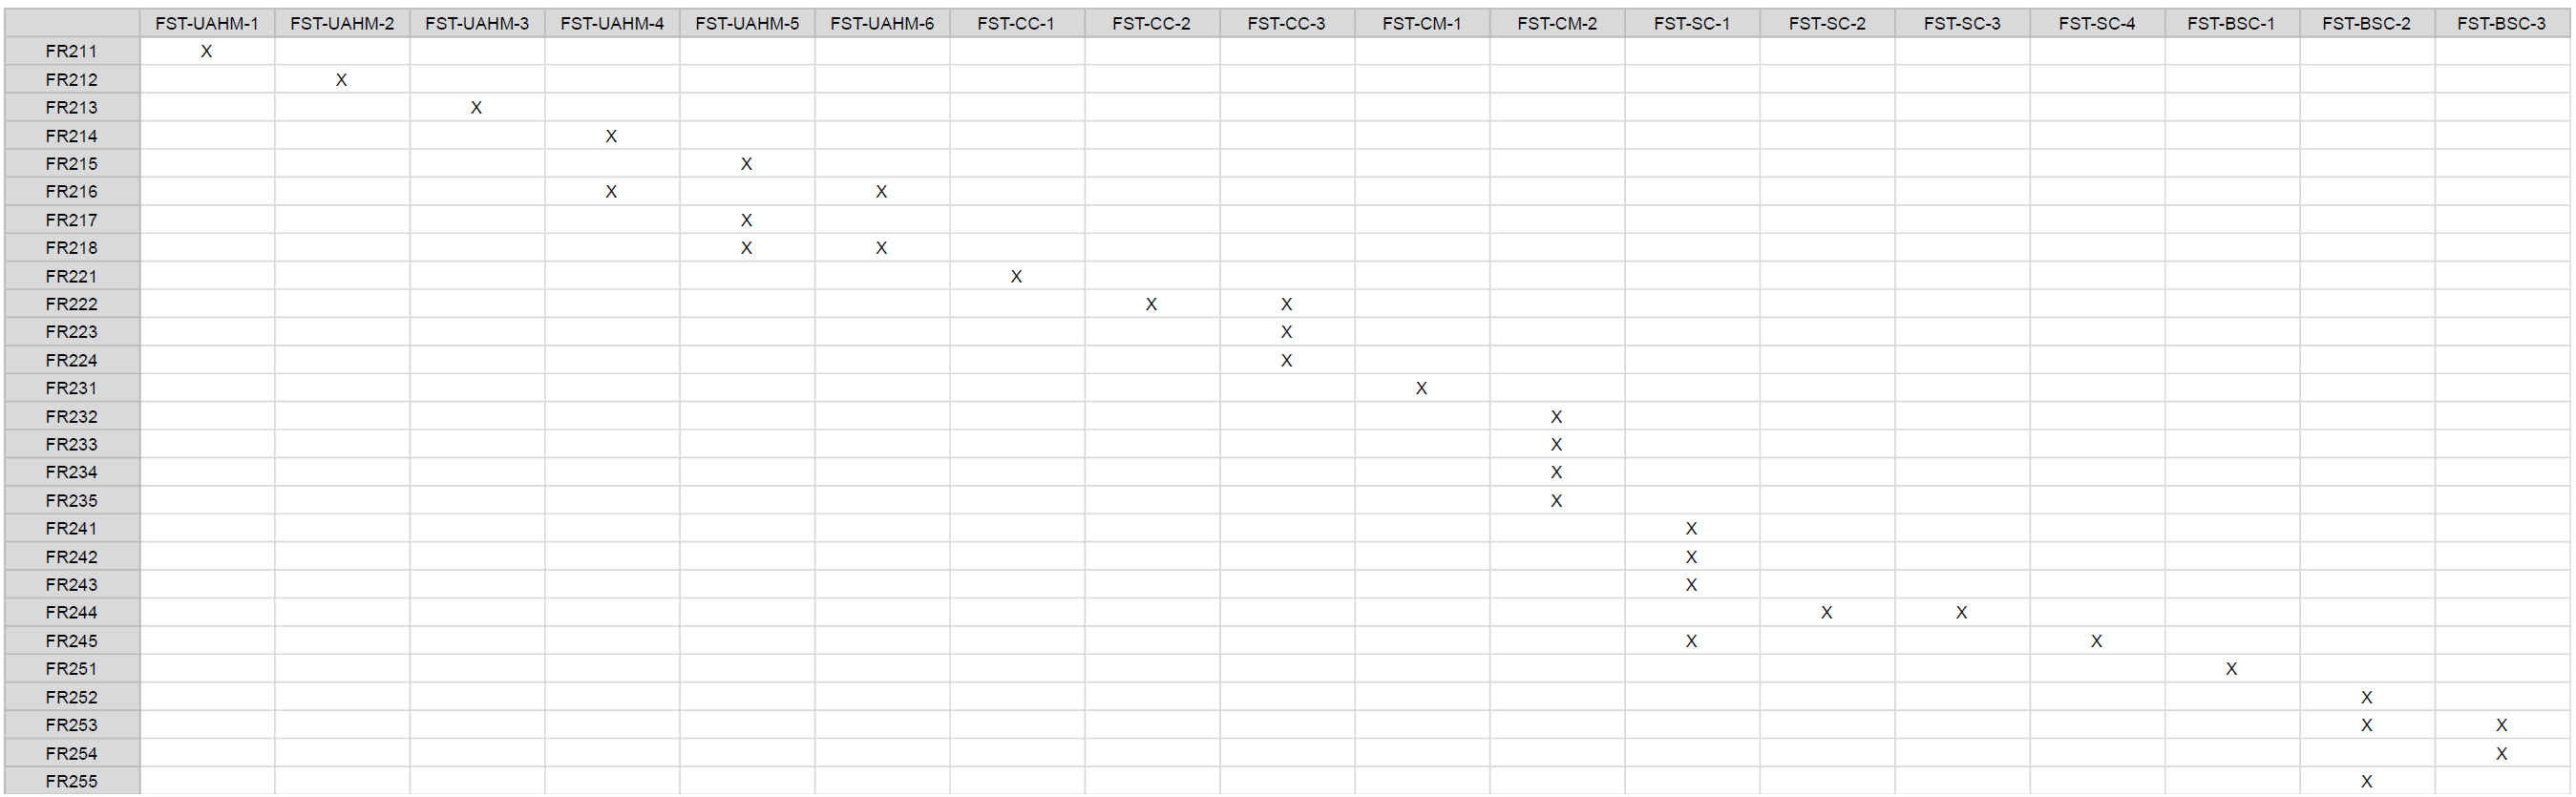
\includegraphics[width=1.4\textwidth]{func_trac_mat.png}}
    \caption{Functional requirements - tests traceability}
    \label{fig:fr}
  \end{figure} 
  
\begin{figure}[h!]
  \makebox[\textwidth][l]{\hspace{-3cm}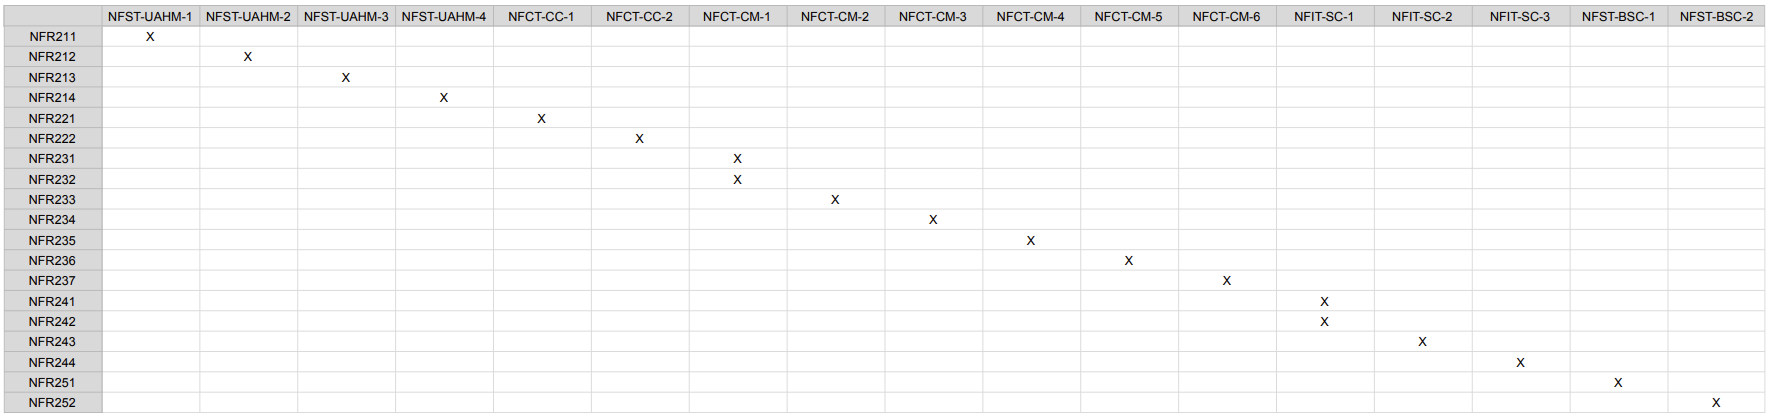
\includegraphics[width=1.4\textwidth]{nonfunc_trac_mat.png}}
  \caption{Non-functional requirements - tests traceability}
  \label{fig:nfr}
\end{figure}
  
 

\section{Unit Test Description}
To be included in future revisions.

\bibliographystyle{plainnat}

\bibliography{../../refs/References}

\newpage

\section{Appendix}

\section*{Appendix --- Reflection}


The information in this section will be used to evaluate the team members on the
graduate attribute of Lifelong Learning.

\input{../Reflection.tex}

\begin{enumerate}
  \item What went well while writing this deliverable? 
  \item What pain points did you experience during this deliverable, and how
    did you resolve them?
  \item What knowledge and skills will the team collectively need to acquire to
  successfully complete the verification and validation of your project?
  Examples of possible knowledge and skills include dynamic testing knowledge,
  static testing knowledge, specific tool usage, Valgrind etc.  You should look to
  identify at least one item for each team member.
  \item For each of the knowledge areas and skills identified in the previous
  question, what are at least two approaches to acquiring the knowledge or
  mastering the skill?  Of the identified approaches, which will each team
  member pursue, and why did they make this choice?
\end{enumerate}
Answers:
\begin{enumerate}
  \item While writing this deliverable, the team was able to start much earlier and each individual member of the team took more initiative. This lead to the deliverable being close to completion much earlier (relative to the deadline) than other deliverables for the project. Additionally, we had planned some questions before our meeting with our TA which when answered gave us a lot of clarity about this deliverable so we were able to  work with less confusion. Finally, the work items for this deliverable were separated very fairly, with the core sections of this deliverable having multiple people working on them and other sections being delegated to a single person.
  \item There were not any major pain points in this deliverable. Some minor pain points that did occur include some confusions about what do with section 3.3 and section 5, as they relate to the design document which at the time of writing, has not been completed. Another minor paint point was that the this document required the SRS to be modified in situtations which we discovered new requirements and since our SRS, this was cumbersome and difficult to coordinate for the multiple group members developing test cases who may have done duplicate work. To deal with this, we created a thread in our group chat on discord where we notified each other when modifications were being done to the SRS.
  \item The team will need to learn how to use various tools and testing libraries to complete the verification of the project. Some of these tools and libraries include the automation of tests on GitHub Actions, testing libraries for specific programming languages (Pytest, Jest, etc), and Postman. In addition to just tools and libraries, the team will also need to learn and improve their analytical skills for software. This project involves a lot of analysis on all aspects of it such as requirements, code, and use cases. Learning and improving the teams code review / walkthrough skills, to effectively evaluate / communicate what the code would / should do is essential.
  \item For learning a new testing tool or library, our team has decided to rely on the countless resources available on the internet, as well as an opportunity for transferable knowledge. Applying these methods will help with integrating automated testing into our software effectively.\\
  One approach for mastering a new tool or library is to follow a tutorial or short course readily available online, for instance this \href{https://www.youtube.com/playlist?list=PLM-7VG-sgbtAgGq_pef5y_ruIUBPpUgNJ}{Intro to Postman} Youtube series or this \href{https://www.linkedin.com/learning/unit-testing-in-python}{Unit Testing in Python} course from LinkedIn Learning. Maged Armanios will use this approach because by following a tutorial created by an expert, he can understand important nuances of the software. In addition, he enjoys following tutorials and learns well when doing a guided lesson.\\
  Another approach is to create a small, simple project for unit testing and using the documentation/reference material from the library chosen, integrate the tool on a small scale and keep increasing the coverage until it is adequate for the entire project. For our project, we will use the proof of concept (POC) as our basic starting point to add test automation, and then expand into other modules as we gain familiarity with the chosen tool. Harshil Patel will lead this effort because he has experience working in software testing and test automation. Harshil's foundation in congruent skills gives him confidence that he can successfully integrate a testing library with just the distributor’s reference material.\\
  Improving software analytical skills will really improve the functionality of the software and ensure the code is concise, optimal, and scalable/maintainable. There are countless approaches to developing these skills but we believe the ones identified below are most applicable to our project.\\
  The first approach would be to gather all the diagrams from all our documentation, and create more as necessary to really harbour the understanding of exactly how the code will be used and how functions will be fulfilled. Such diagrams include case diagrams, sequence diagrams, and flow charts. This is delegated to Zayn Abed because Zayn is strong with organization and attention-to-detail. He will be able to lay out the flow and functionality of the app and ensure there are no gaps.\\
  The second approach expands on the first one, and it is to use the findings to draw common themes and create a software architecture that incorporates design patterns to accomplish the purpose of each module. Material from previous courses will be used to aid in ultimately creating a UML diagram that encapsulates our software. Using design patterns and principles will ensure scalability, reusability, modularity, testability, and more qualities of good design. Jane Klavir will follow this approach because Jane is passionate about design and bringing together individual parts to make a cohesive whole.\\
  A third approach is to conduct code walkthroughs for our supervisor, Dr. Tharmarasa, as new elements are implemented. While these walkthroughs do not have to be perfect or formal, they should clearly get the point across to our supervisor so that he can analyse the software effectively and provide his expert evaluation. Jinal Kasturiarachchi will be responsible for doing walkthroughs in meetings with Dr. Tharmarasa because Jinal enjoys presenting and opening the discussion for team to furthermore receive valuable feedback.  \\
\end{enumerate}

\end{document}